\documentclass{article}

\usepackage{style}

\lhead{MEEN 612: Project}
\rhead{Bryan Yaggi}

\begin{document}

\section{Mechanical Design}

The manipulator is 7R spatial.
The design is inspired by the human arm.
It only possesses single degree-of-freedom joints,
but the three joints representing the shoulder, two joints representing the elbow, and two joints representing the wrist
are in close proximity.
The shoulder, elbow, and wrist joint groups are separated by longer links.
Also, neighboring joint axes intersect.
The result is a manipulator like the Kuka LBR iiwa.

The manipulator was modeled in Solidworks.
Each link with exception to the base and end are configurations of the same part.
Each joint uses the same hardware.
This modularity is inspired by the CMU snake robot.
The joint is designed so the shaft is fixed with respect to one link and rotates with respect to the other on plain
bearings.
The shaft is a hex head screw, and the axial play is controlled with a locknut.
\autoref{table:bom} is the bill of materials.

\begin{table}[h]
\begin{center}
\caption{Bill of materials.}
\label{table:bom}
\begin{tabular}{|r|l|l|r|}
  \hline
  Line & Description & Quantity \\
  \hline
  1 & Base & 1 \\
  2 & Link 1 & 1 \\
  3 & Link 2 & 3 \\
  4 & Link 3 & 2 \\
  5 & End & 1 \\
  6 & 1/4"-20 x 2.25" Hex Head Screw (McMaster-Carr 91257A551) & 7 \\
  7 & 1/4"-20 Nylon-Insert Locknut (McMaster-Carr 94945A205) & 7 \\
  8 & Plain Bearing, 1/4" Shaft, 3/8" Housing, Flanged (McMaster-Carr 1677K1) & 14 \\
  \hline
\end{tabular}
\end{center}
\end{table}

The links were printed on my personal Prusa i3 MK3S+ printer.
The links are in alternating colors -- including Aggie maroon -- to better visualize the joints.
The manipulator is currently at my desk in the Research Integration Center (RIC) at TAMUS RELLIS.

\begin{figure}[H]
  \centering
  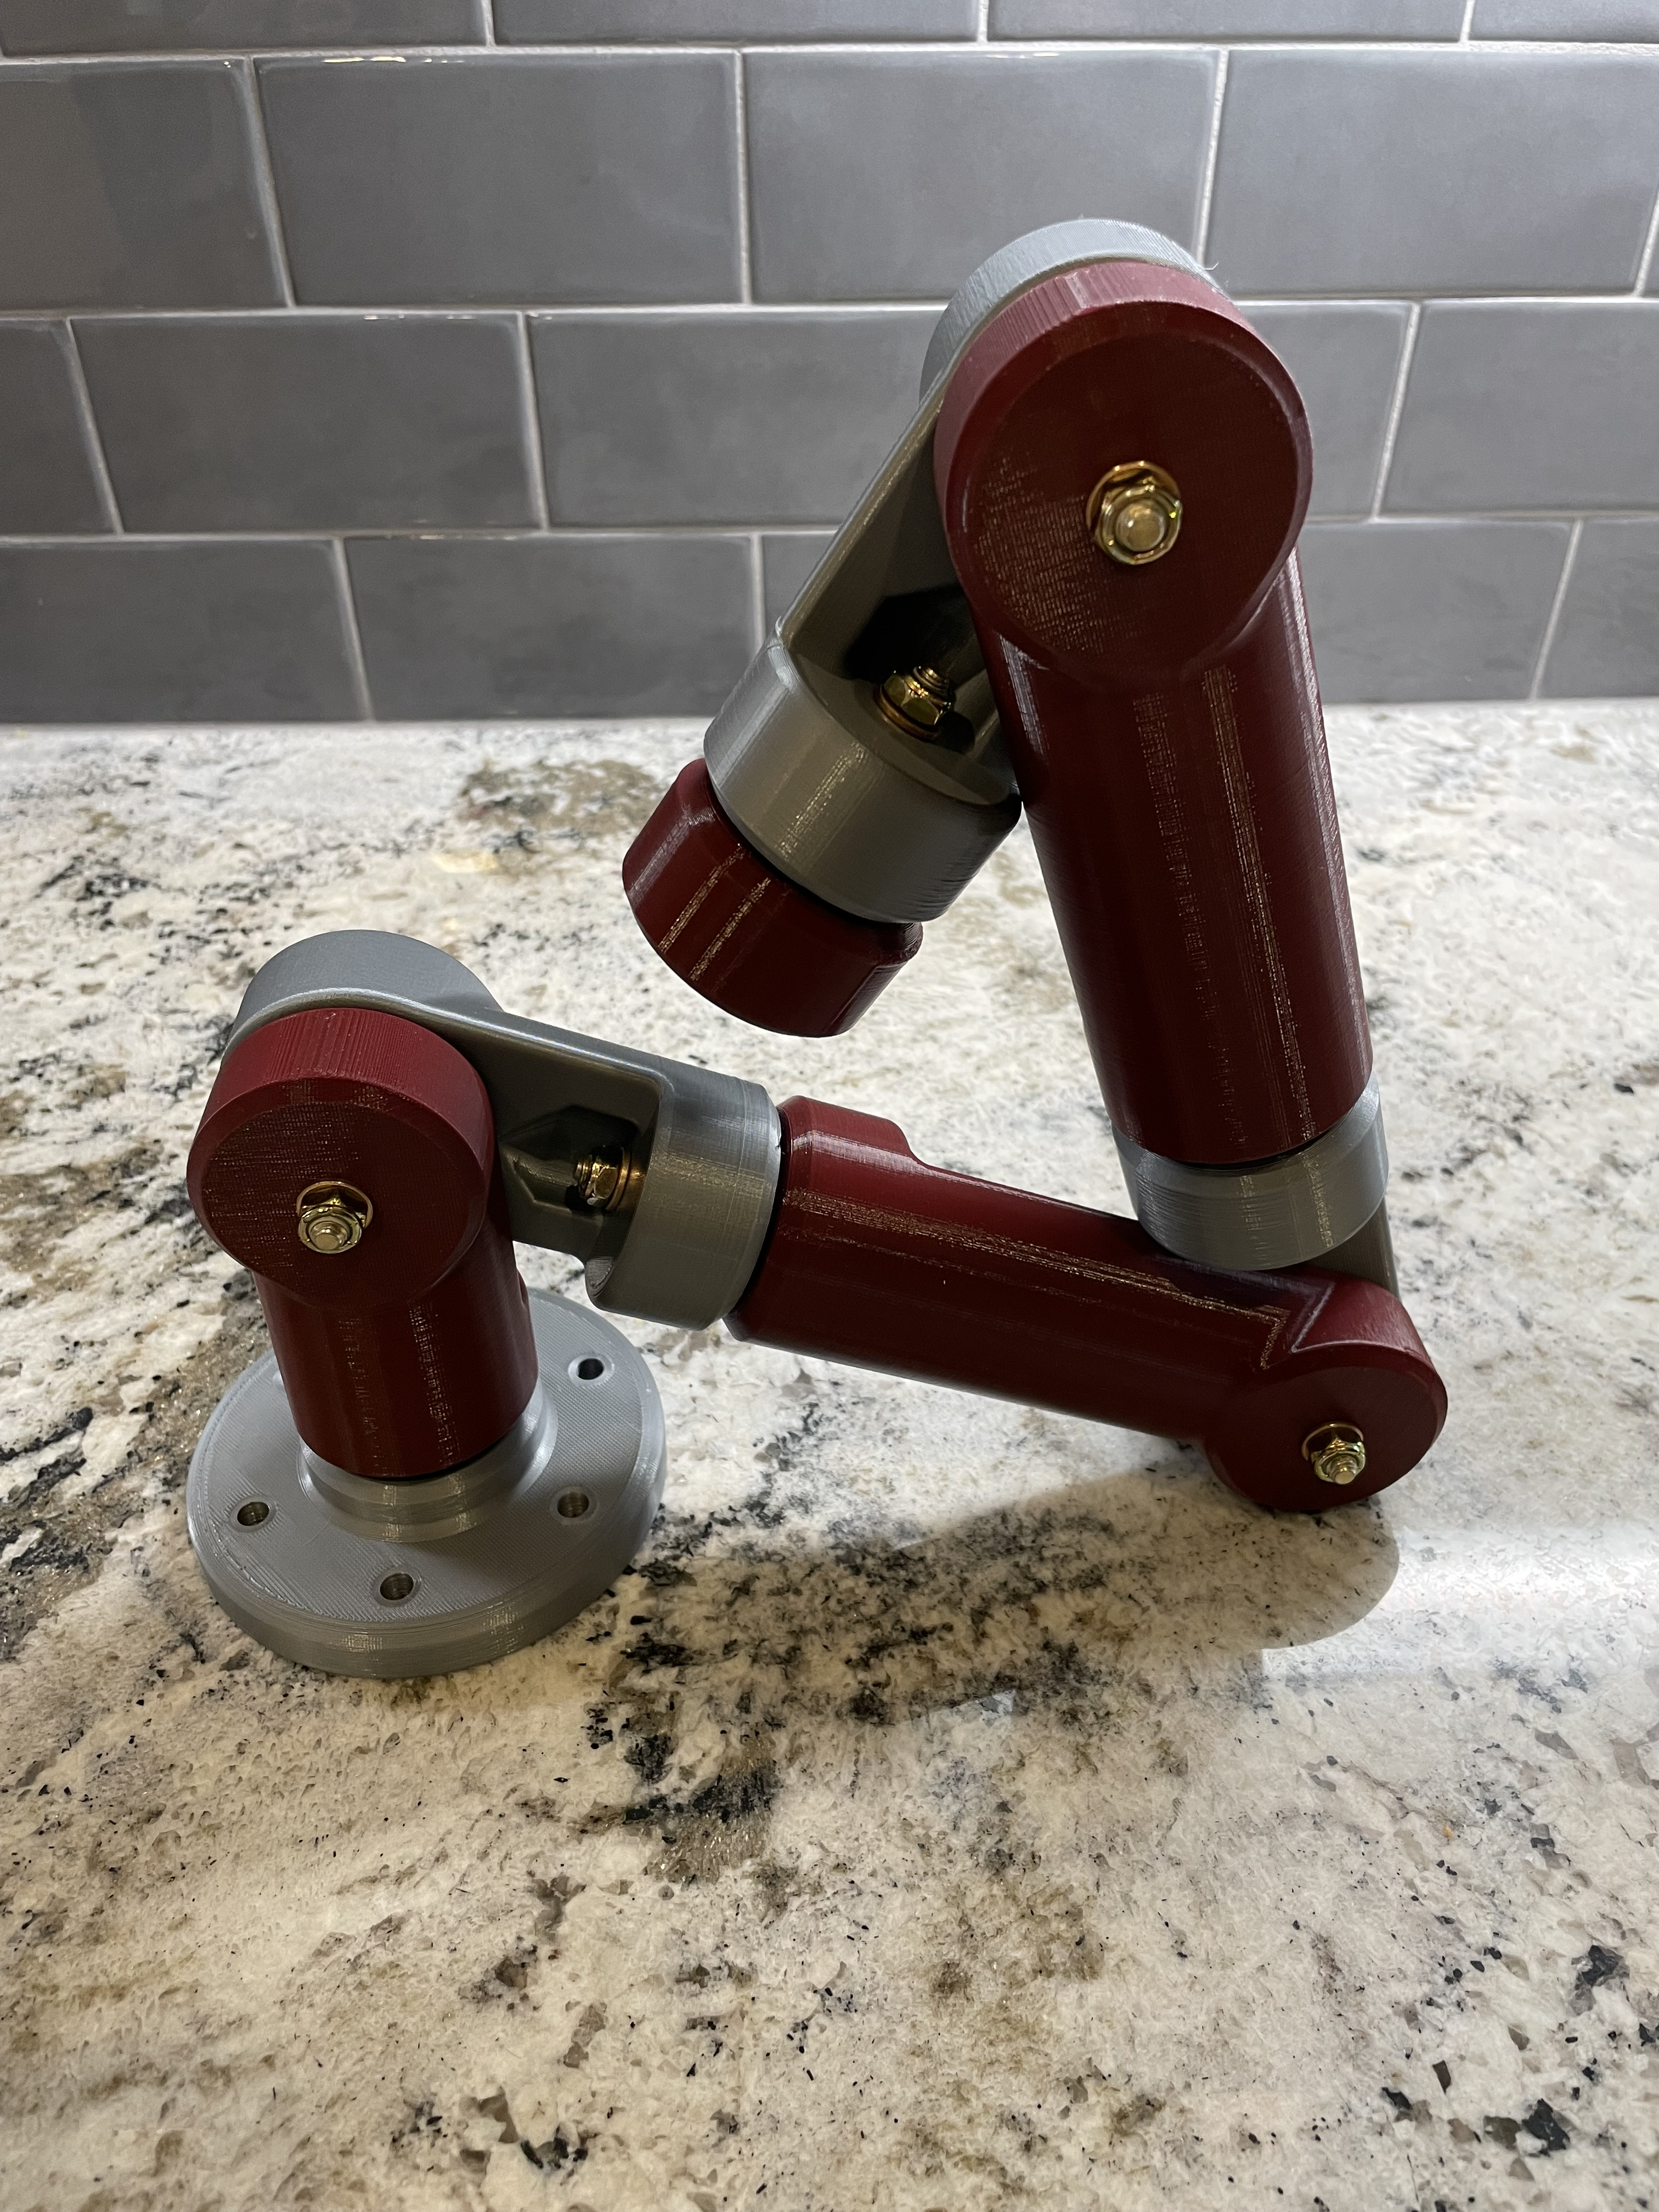
\includegraphics[width=0.3\linewidth]{counter1}
  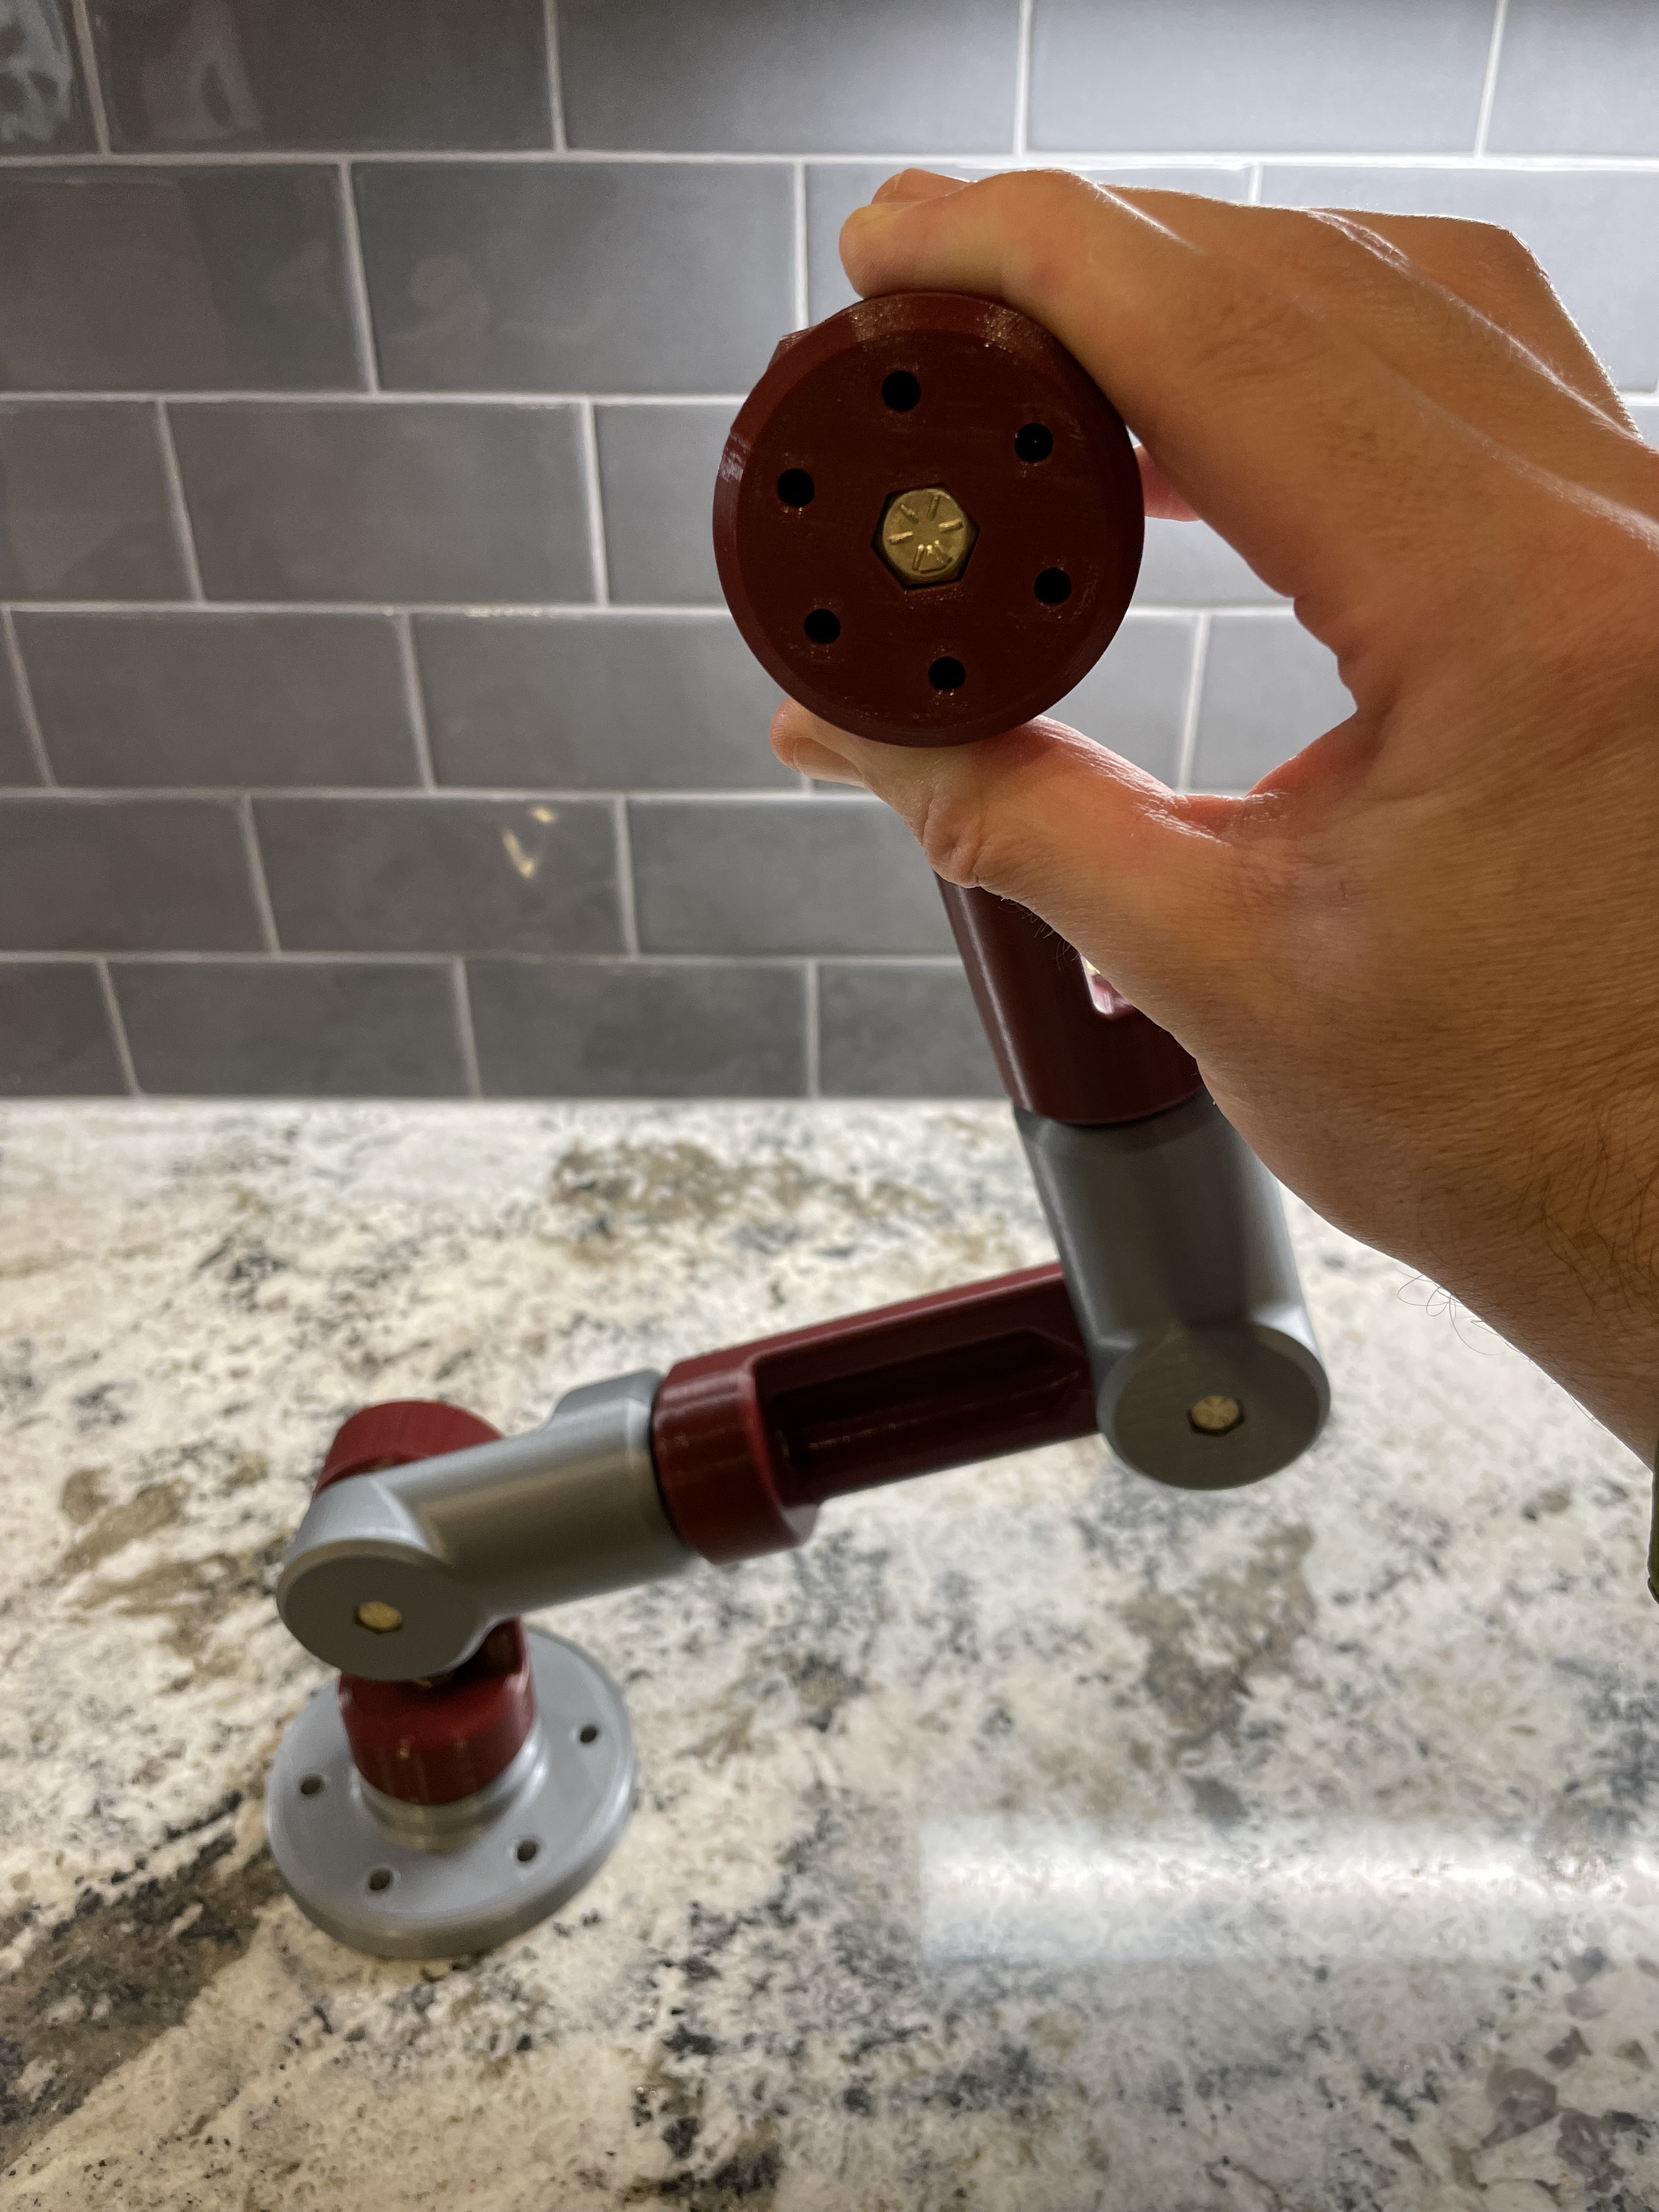
\includegraphics[width=0.3\linewidth]{counter2}
  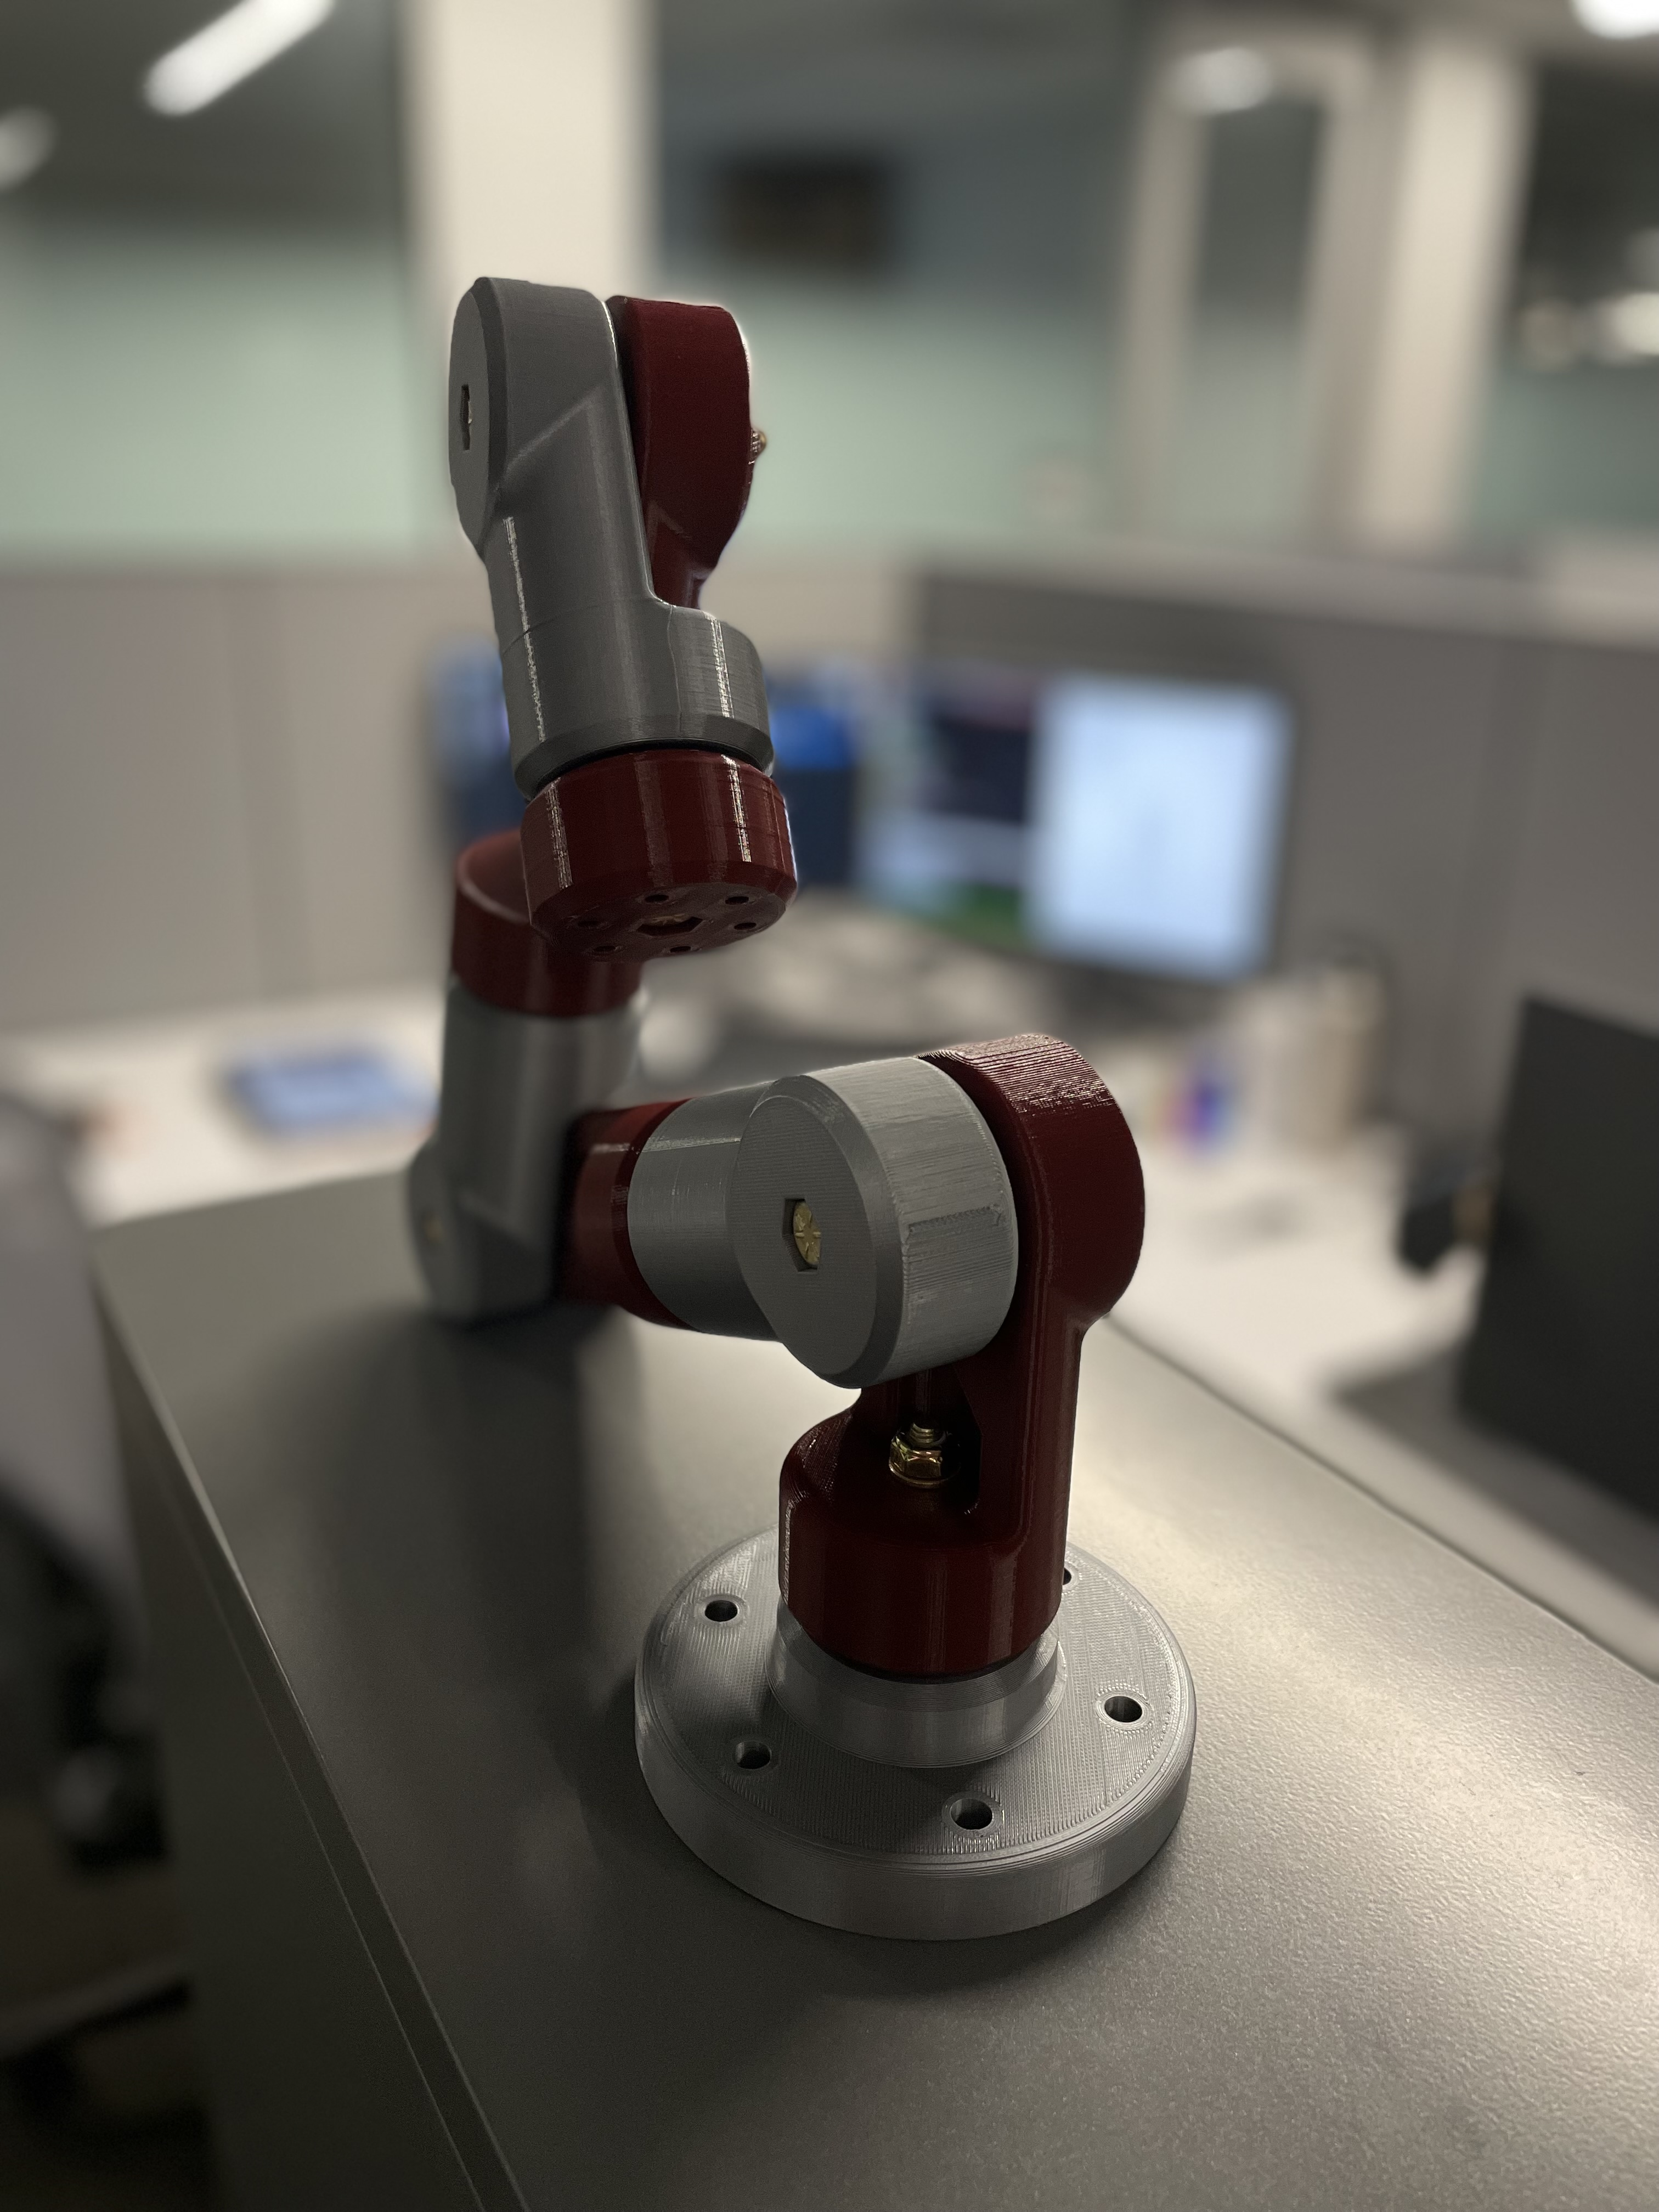
\includegraphics[width=0.3\linewidth]{ric1}
  \caption{Physical manipulator. Right image shows the manipulator at my desk at the RIC.}
\end{figure}

\pagebreak
\section{Kinematics}

Coordinate frames were defined in Solidworks using modified D-H parameters.
These coordinate frames were used with the Solidworks to URDF exporter add-in so the URDF would be defined with the D-H
frames.
\autoref{fig:frames} shows the frames.
Even and odd frames are shown in different subfigures for better visualization.
\autoref{table:dh} shows the corresponding modified D-H parameters.
    
\begin{figure}[h]
  \centering
  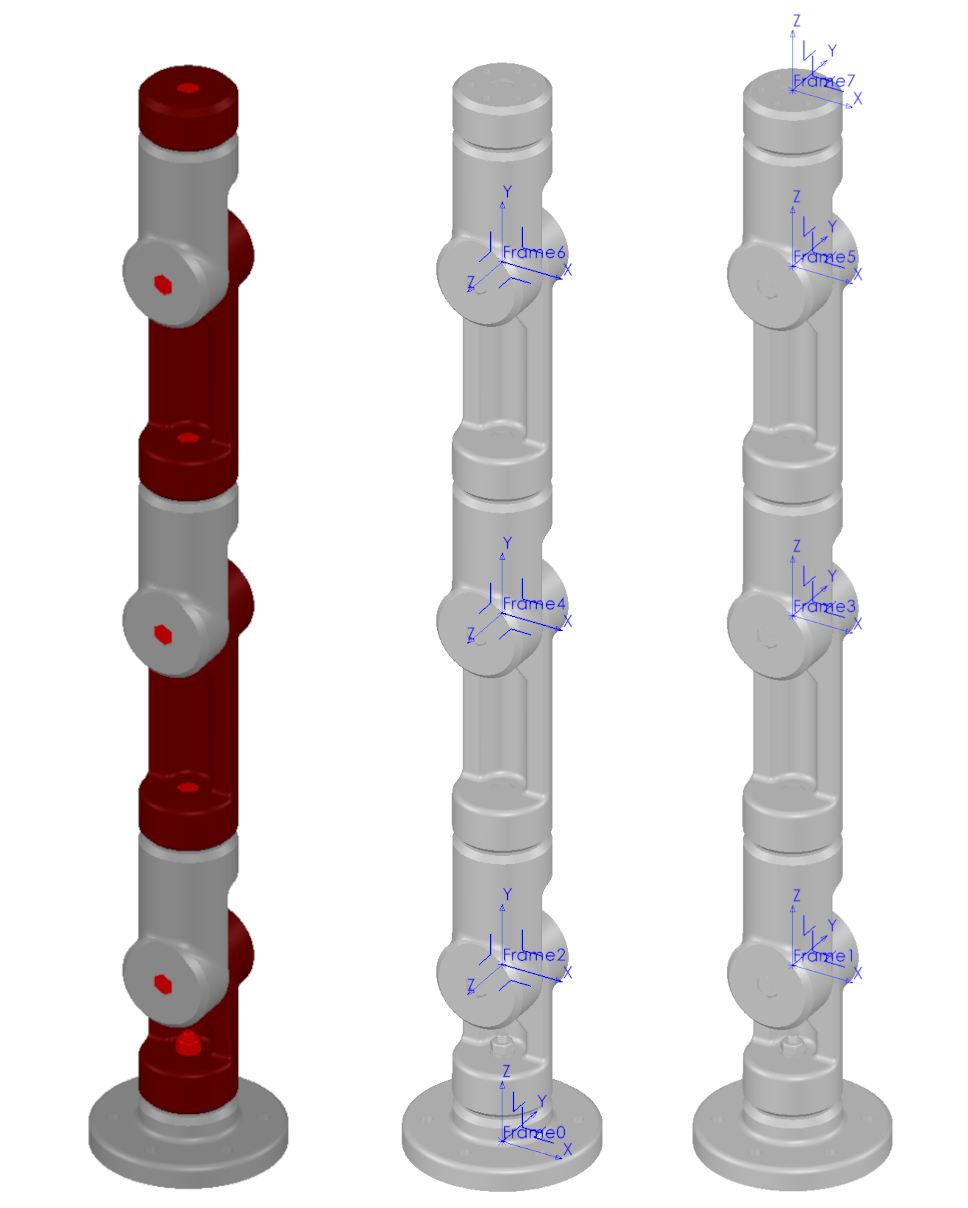
\includegraphics[height=0.5\linewidth]{dhFrames}
  \caption{Frame definitions. Middle subfigure shows even frames. Right subfigure shows odd frames.}
  \label{fig:frames}
\end{figure}

\begin{table}[h]
\begin{center}
\caption{Modified D-H parameters.}
\label{table:dh}
\begin{tabular}{|c c c c c|}
  \hline
  Joint $i$ & $\alpha_{i-1}$ & $a_{i-1}$ & $d_i$ & $\theta_i$ \\
  \hline
  1 & $0^\circ$ & 0 & $l_1 + b + l_2$ & $q_1$ \\
  2 & $90^\circ$ & 0 & 0 & $q_2$ \\
  3 & $-90^\circ$ & 0 & $l_2 + b + l_3$ & $q_3$ \\
  4 & $90^\circ$ & 0 & 0 & $q_4$ \\
  5 & $-90^\circ$ & 0 & $l_2 + b + l_3$ & $q_5$ \\
  6 & $90^\circ$ & 0 & 0 & $q_6$ \\
  7 & $-90^\circ$ & 0 & $l_2 + b + l_1$ & $q_7$ \\
  \hline
\end{tabular}
\end{center}
\end{table}
In \autoref{table:dh}, $b = \frac{1}{16}"$ is the plain bearing flange thickness,
$l_1 = 1"$, $l_2 = 3"$, and $l_3 = 5"$.

The transforms between each frame necessary for forward kinematics are calculated below.
\begin{align}
  \p{0}{1}T &= \begin{bmatrix}
    cq_1 & -sq_1 & 0 & 0 \\
    sq_1 & cq_1 & 0 & 0 \\
    0 & 0 & 1 & l_1 + b + l_2 \\
    0 & 0 & 0 & 1
  \end{bmatrix} = \begin{bmatrix}
    cq_1 & -sq_1 & 0 & 0 \\
    sq_1 & cq_1 & 0 & 0 \\
    0 & 0 & 1 & 4.0625 \\
    0 & 0 & 0 & 1
  \end{bmatrix} \\
  \p{1}{2}T = \p{3}{4}T = \p{5}{6}T &= \begin{bmatrix}
    cq & -sq & 0 & 0 \\
    0 & 0 & -1 & 0 \\
    sq & cq & 0 & 0 \\
    0 & 0 & 0 & 1
  \end{bmatrix} = \begin{bmatrix}
    cq & -sq & 0 & 0 \\
    0 & 0 & -1 & 0 \\
    sq & cq & 0 & 0 \\
    0 & 0 & 0 & 1
  \end{bmatrix} \\
  \p{2}{3}T = \p{4}{5}T &= \begin{bmatrix}
    cq & -sq & 0 & 0 \\
    0 & 0 & 1 & l_2 + b + l_3 \\
    -sq & -cq & 0 & 0 \\
    0 & 0 & 0 & 1
  \end{bmatrix} = \begin{bmatrix}
    cq & -sq & 0 & 0 \\
    0 & 0 & 1 & 8.0625 \\
    -sq & -cq & 0 & 0 \\
    0 & 0 & 0 & 1
  \end{bmatrix} \\
  \p{6}{7}T &= \begin{bmatrix}
    cq_7 & -sq_7 & 0 & 0 \\
    0 & 0 & 1 & l_2 + b + l_1 \\
    -sq_7 & -cq_7 & 0 & 0 \\
    0 & 0 & 0 & 1
  \end{bmatrix} = \begin{bmatrix}
    cq_7 & -sq_7 & 0 & 0 \\
    0 & 0 & 1 & 4.0625 \\
    -sq_7 & -cq_7 & 0 & 0 \\
    0 & 0 & 0 & 1
  \end{bmatrix}
\end{align}
where $q = q_i$ for $\p{i-1}{i}T$ and $s$ and $c$ represent $\sin$ and $\cos$, respectively.

\pagebreak
\section{Control}

\subsection{Description}

A computed torque controller is implemented. \autoref{fig:ctd} is a diagram of the controller.
\begin{figure}[h]
  \centering
  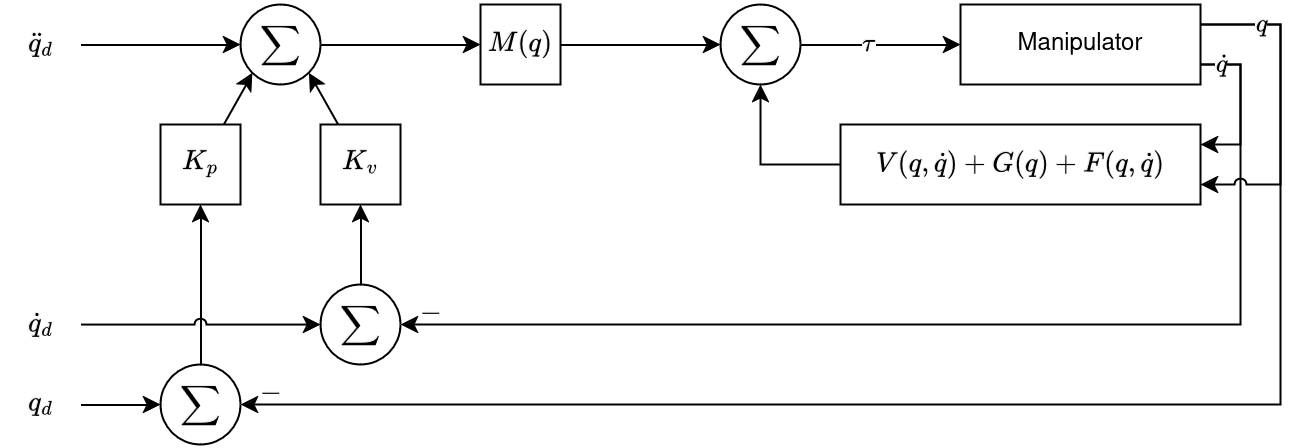
\includegraphics[width=0.75\linewidth]{computed_torque_diagram}
  \caption{Computed torque diagram.}
  \label{fig:ctd}
\end{figure}
The manipulator dynamics are
\begin{align}
  M(q)\ddot{q} + V(q, \dot{q}) + G(q) + F(q, \dot{q}) = \tau
\end{align}
where $M$ is the inertia matrix, $V$ contains centrifugal and Coriolis terms, $G$ contains gravity terms, and $F$
contains friction terms. The control law is
\begin{align}
  \tau = M(q)[\ddot{q}_d + K_v(\dot{q}_d - \dot{q}) + K_p(q_d - q)] + V(q, \dot{q}) + G(q) + F(q, \dot{q})
\end{align}
The controller cancels the nonlinear dynamics and adds proportional and derivative error terms.
The resulting closed-loop dynamics are
\begin{align}
  \ddot{E} + K_v \dot{E} + K_p E = 0 \label{eq:cld}
\end{align}
where $E = q_d - q$. This is a linear second-order system.

\subsection{Stability}

Since the computed torque controller produces a closed-loop linear second-order system, the system is stable if the
gains are chosen such that the roots have negative real components.
For the implemented controller, gains are chosen to achieve critical damping:
\begin{align}
  K_v = 2 \sqrt{K_p}
\end{align}

Stability can also be proven using Lyapunov. A candidate Lyapunov function is
\begin{align}
  v = \frac{1}{2} \dot{E}^\top \dot{E} + \frac{1}{2} E^\top K_p E \succ 0
\end{align}
This function is positive definite since $K_p$ is positive definite. Additionally,
\begin{align}
  v = \begin{bmatrix}
    E \\
    \dot{E}
  \end{bmatrix}^\top \begin{bmatrix}
    K_p & 0 \\
    0 & I
  \end{bmatrix} \begin{bmatrix}
    E \\
    \dot{E}
  \end{bmatrix} > \beta \begin{Vmatrix}
    E \\
    \dot{E}
  \end{Vmatrix}^2
\end{align}
where $\beta = \min(\lambda_{K_p, \min}, 1)$ and $\lambda_{K_p, \min}$ is the minimum eigenvalue of $K_p$. The
derivative of the candidate function is
\begin{align}
  \dot{v} = \dot{E}^\top \ddot{E} + E^\top K_p \dot{E}
\end{align}
Plugging in the system dynamics $\ddot{E} = -K_v \dot{E} - K_p E$,
\begin{equation}
\begin{aligned}
  \dot{v} &= \dot{E}^\top (-K_v \dot{E} - K_p E) + E^\top K_p \dot{E} \\
          &= -\dot{E}^\top K_v \dot{E} \preceq 0
\end{aligned}
\end{equation}
The derivative is negative semi-definite since $K_v$ is positive definite.
Steady-state analysis showing the system cannot get stuck away from the fixed point is needed to prove asymptotic
stability by LaSalle's Theorem.
The system can only get stuck if $\ddot{E} = \dot{E} = 0$,
which requires $E = 0$ from \eqref{eq:cld}.
Therefore, the system is asymptotically stable.

\subsection{Simulation}

The manipulator was simulated using PyBullet.
I wanted to use an environment other than MATLAB;
I have used it in industry, but research seems to favor Python and simulators like PyBullet and MuJoCo seem more popular.
I used the student version of CoppeliaSim for another robotics course,
so I wanted to experiment with something else.
I initially tried using the Python Robotic Toolbox developed by the lead developer of MATLAB's Robotics Toolbox,
Peter Corke.
While most of the functionality worked,
the package was unusable because of a bug in getting the mass matrix from a robot imported via URDF.
\footnote{\href{https://github.com/petercorke/robotics-toolbox-python/issues/368}{GitHub issue}}
There were other issues too, such as not being compatible with the latest release of SciPy.

The following are links to the flopping videos:
\begin{itemize}
  \item \href{./downflop_bullet.mp4}{downflop\_bullet.mp4}
  \item \href{./upflop_bullet.mp4}{upflop\_bullet.mp4}
\end{itemize}
The flopping videos were also created using MATLAB before the PyBullet simulation was working.

\autoref{fig:impulse} is an impulse response plot created by perturbing each joint with a large torque at the 2 second
mark while under position regulation control.
The following is a link to the video of the scenario used for creating the plot: \href{./impulse.mp4}{impulse.mp4}.
\begin{figure}[h]
  \centering
  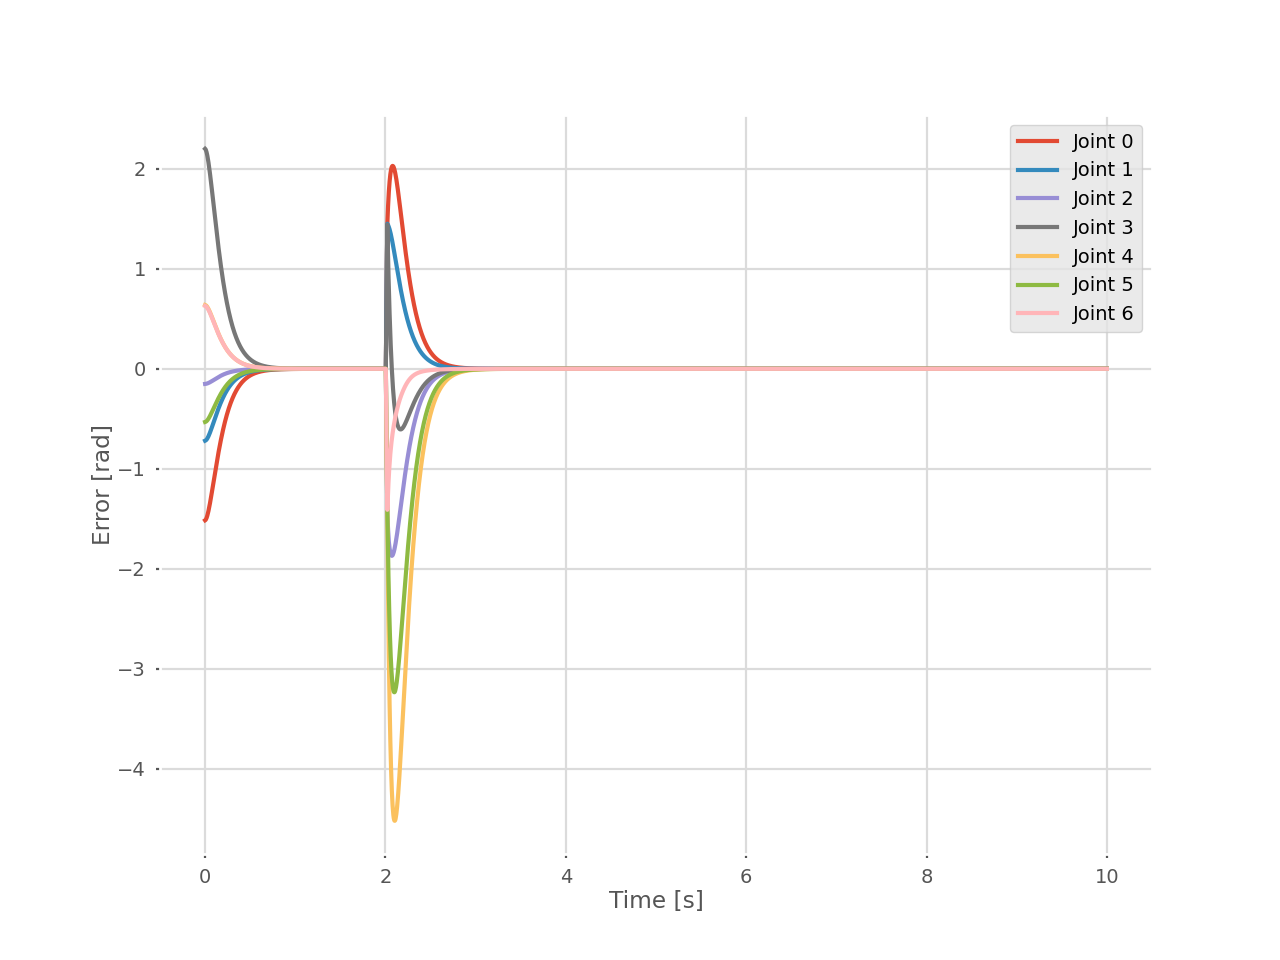
\includegraphics[width=0.6\linewidth]{impulse}
  \caption{Impulse response.}
  \label{fig:impulse}
\end{figure}
The non-zero error at the beginning of the plot is due to the initial movement of the manipulator to the desired
Cartesian pose.

\autoref{fig:ctyz} and \autoref{fig:ct} are plots of the manipulator's path when trying to draw a pentagram in a plane
normal to the x-axis.
The following is a link to the video of the scenario used for creating the plot:
\href{./cartesian\_trajectory.mp4}{cartesian\_trajectory.mp4}
\begin{figure}[h]
  \centering
  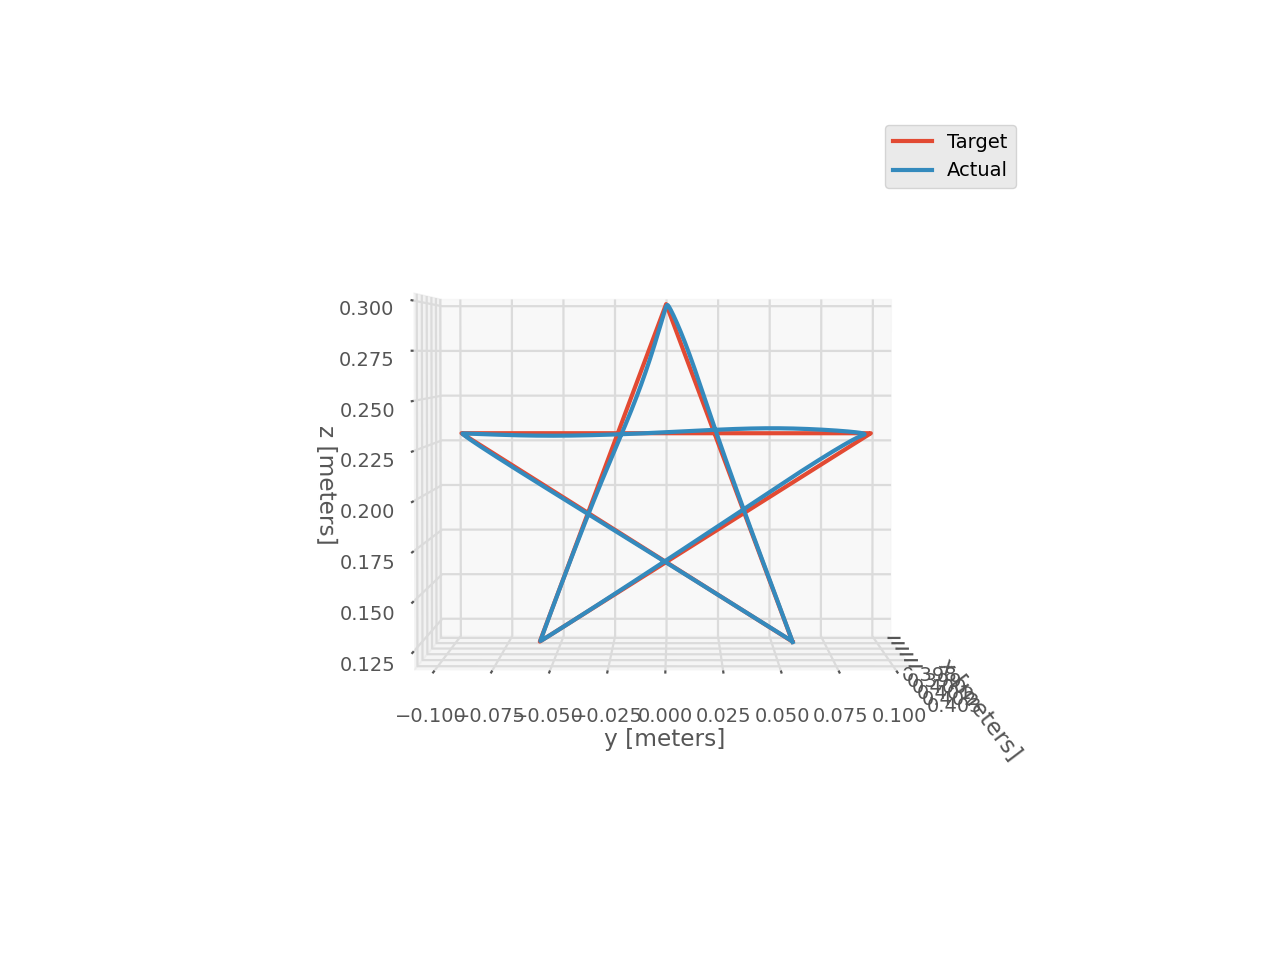
\includegraphics[width=0.6\linewidth]{cartesian_trajectory_yz}
  \caption{Cartesian path viewed normal to plane of pentagram.}
  \label{fig:ctyz}
\end{figure}
\begin{figure}[h]
  \centering
  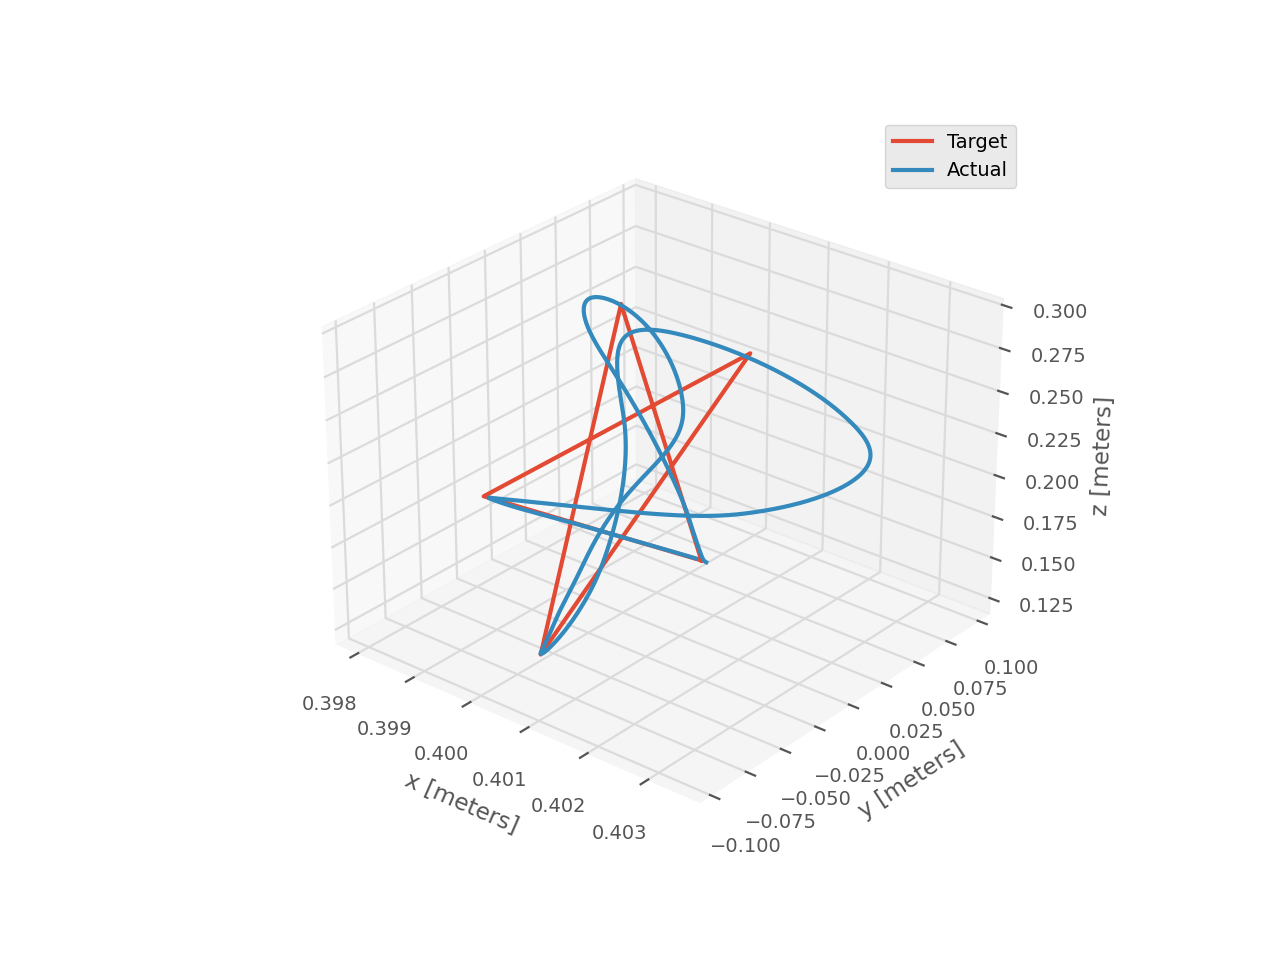
\includegraphics[width=0.6\linewidth]{cartesian_trajectory}
  \caption{Cartesian path in 3D.}
  \label{fig:ct}
\end{figure}
In the figures, the target path is red and the actual path is blue.
The error is much greater along the x-axis, but the maximum error is less than 3 mm.

\end{document}
